\chapter{Ionomics of the Andosol Introgression Resource Panel: Kernel Nutrient Accumulation and Potential Adaptations to Highland and Lowland Phosphorus Deficiencies}
\label{chap-four}

\newrefsection

\section{Abstract}

 Distinct physical and chemical properties might result in the same nutrient limitations for plants growing in different soils.
 For example, because of their volcanic composition, Andosols typically have high total phosphorus, but at the same time a high phosphorus retention, which results in scarce plant available phosphorus, and makes them sub-optimal soils for agriculture. 
 Acrisols, with a sedimentary composition, have a high clay content which also results in low phosphorus availability for plants.
 In this study, I use plants bred in these two types of soils to investigate the genetic causes of adaptation to low phosphorus availability coming from highland and lowland locations.
 For this, I use a population of BC$_2$S$_3$ maize recombinant inbred lines of Mexican andosol donors backcrossed into CML530, an inbred selected for acrisols and ferralsols in Colombia.
 I obtained data for the kernel concentrations of 14 minerals, and I detected  12 quantitative loci for 7 minerals, explaining between 1.8 to 17\% of the observed variance in the traits.
 Phosphorus and manganese kernel content are linked to \textit{Zm00001eb076150}, a locus in chromosome 2 spanning a maize homolog of \textit{WAT1} an auxin transporter in
\textit{Arabidopsis}, among other genes. 
\textit{Zm00001eb076150} has been previously associated, under low phosphorus conditions,  to leaf number in maize and shoot dry weight in wheat, suggesting a plausible gene candidate. 

\section{Background}

\subsection{Phosphorus Restrictions in Andosols}

Andosols, according to WRB system \citep{wrb2022}, or Andisols in the USDA soil taxonomy \citep{scheffe2015, krasilnikov2013}, are soils of volcanic origin that support maize crops, pasture grasses, and native forests in the highlands of Mexico \citep{bayuelo-jimenez2020,galvan-tejada2014}. Maize has been cultivated in the Mexican highlands for the last 6500 years \citep{piperno2001} without industrial fertilizers. Local corn varieties grown in the Andosols of the highland plateau of the Transmexican Volcanic Belt (TMVB) have increased phosphorus use efficiency and higher P acquisition capability, demonstrating adaptation to limiting phosphorus conditions \citep{bayuelo-jimenez2011,bayuelo-jimenez2014}.

Because they tend to retain phosphates, Andosols' productivity is constrained by the amount of the remaining soluble phosphorus available for plant intake.
Out of all 14 USDA soil taxonomy orders, Andosols have the highest global median total phosphorus content with 883,7 ppm [mg P/kg dry soil]\citep{hexianjin2022}.
In contrast, the median available phosphorus, measured by the Bray-1 test method \citep{bray1945}, is 2.6 ppm for natural Andosol Mexican topsoils (calculated from \cite{paz-pellat2018}). 
In the US, the critical concentration recommended for growing commercial corn varieties with optimal yield is 15 ppm of Bray-1 P \citep{lyons2023}, and soil concentrations of 10 ppm Bray-1 P can cause loses of up to 50\% in yield \citep{dodd2005}.
Thus, the typical natural Mexican andosol is phosphorus deficient relative to modern corn agriculture standards. 

Volcanic glass is the source of the Andosols’ high content of alumino-silicate and ferrihydrites that transform over time into allophanes and imogolites \citep{wrb2022}
These minerals make Andosols highly acidic soils and confer a high cation exchange capacity due to their high surface area and large number of reactive sites\citep{krasilnikov2013}.
In these acidic conditions, aluminum and iron cations promote complexes that precipitate phosphates from the soil solution and strongly bind them to the soil particles \citep{krasilnikov2013}. Plant adaptations that allow the extraction of these occluded minerals might increase plant phosphorus acquisition efficiency. 


\subsection{Genotype by Environment interaction determines kernel phosphorus  accumulation strategies.}

In modern hybrids, almost 80\% Of the total plant phosphorus uptake is accumulated in the seed as post-silking uptake, a proxy for direct soil uptake, under optimal agronomic conditions \citep{bender2013}. 
However, the strategies for P acquisition and kernel accumulation are dependent on phosphorus availability, the plant genotype, and their interaction as illustrated by two Tropical/subtropical inbreds in \citep{sun2023}. 
In that study, the inbred CIMBL89 grown in low phosphorus acquires 87.4\% of seed P from post-silking uptake, while in high phosphorus 94\% of seed P is remobilized from other tissues (60\% coming just from the stalks).
In stark contrast, the inbred CML118 has the opposite strategy, under low phosphorus it accumulates 91.1\% of its seed phosphorus from tissue remobilization (38.6\% coming from lower leaves), and in high phosphorus, it acquires 76.4\% of kernel P directly from post-silking uptake. 
Coincident with the pattern of later P acquisition under low phosphosphorus,  the CML118 root/shoot ratio at maturity is greater than in CIMBL89. 
Thus, the genetic analysis of diverse germplasm with potentially different kernel nutrient accumulation strategies can contribute to revealing the genetic architecture of mineral kernel content.

\subsection{QTLs controlling ionomics in the maize kernel}

Single-kernel ionomics is a valuable approximation for investigating the genetic basis of seeded nutrient accumulation in corn. 
In a multi-environment experiment with B73 $\times$ Mo17 recombinant inbred lines, broad sense heritabilities varied from 0.3 (P) to 0.87 (Ca), 27 QTLs where found for ten different minerals, and the amount of variance explained by the significant QTLs varied between 0.04 (P) and 0.27 (K) \citep{baxter2013}. 
In an experiment with the B73 x IL14H population \citep{baxter2014}, the narrow sense heritabilities in single environments varied between 0.28 (Na) and 0.81 (P). In another multi-environment experiment of B73 $\times$ Mo17 RILs \citep{asaro2016} found 79 quantitative trait loci determining the seed content of 20 minerals, including phosphorus. 
Mineral content in single kernels shows enough heritability to be amenable to genetic analysis in the search for candidate loci.

\subsection{Exploring the genetics of adaptation to two kinds of acid soils with high phosphorus retention}
In this work, we use ionomics to search for quantitative trait loci for kernel mineral content, including phosphorus, in a segregating population as a step to understand the genetic basis of kernel mineral composition underlying nutrient use efficiency.
Our maize mapping population has been derived from 15 founder landraces native to  Andosols collected in the Transmexican Volcanic Belt (TMVB) and the Sierra Madre of Chiapas and Guatemala (SMCG).
These donors were crossed to the recurrent parent  CML530, a tropical inbred selected for adaptation to acid soils in Colombia.
In contrast to the Andosol donors, CML530 was bred in a humic acrisol at Andean mid-elevations (Santander de Quilichao, 1000 masl) and tested in a haplic ferralsol of the lowland Orinoco plains (Carimagua) \citep{granados1995}.
Therefore, these crosses might combine different phosphorus acquisition and phosphorus use efficiency strategies in maize, the donor landraces conferring adaptation to andosols, and CML530, adaptation to acrisols.

\begin{figure}[!ht]
\centering
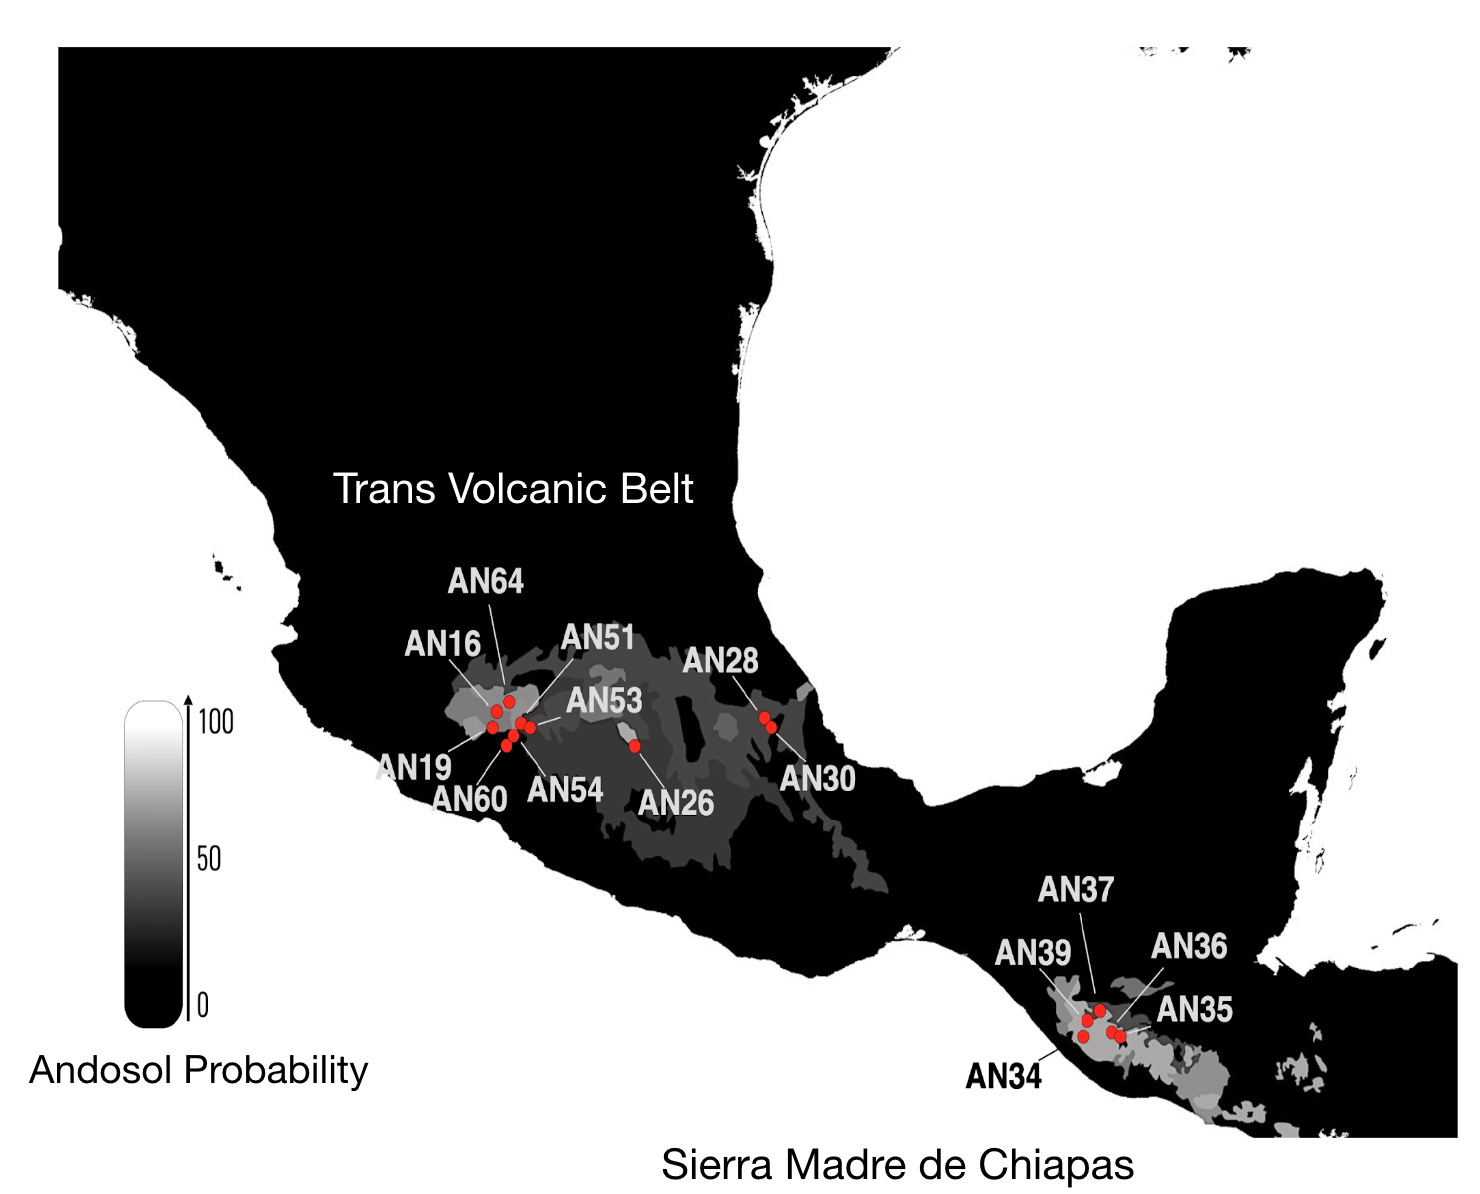
\includegraphics[width=\linewidth]{Chapter-4/figs/parentmap.png}
\caption[Geographic Distribution of AIR Panel Andosol Founders]
{\textit{\textbf{Geographic Distribution of AIR Panel Andosol Donors.}}
15 landraces were selected from Mexico and Guatemala Andosols to be founders of the populations.}
\label{fig::parentmap}
\end{figure}

\clearpage

% Please add the following required packages to your document preamble:
% \usepackage{booktabs}
% \usepackage{graphicx}
\begin{table}[]
\caption{Andosol Introgression Resource Donors,  Traditional Varieties.}
\label{tab::donordata}
\resizebox{\textwidth}{!}{%
\begin{tabular}{@{}llllrrrlr@{}}
\toprule
\textbf{Code} &
  \textbf{Accession} &
  \textbf{Collection} &
  \textbf{Mountain Range} &
  \multicolumn{1}{l}{\textbf{Latitude}} &
  \multicolumn{1}{l}{\textbf{Longitude}} &
  \multicolumn{1}{l}{\textbf{Elevation}} &
  \textbf{Primary race} &
  \multicolumn{1}{l}{\textbf{Families}} \\ \midrule
AN16 & MICH 329 & CIMMYT  & TMVB  & 19.68 & -101.97 & 2292 & Conico               & 101   \\
AN19 & MICH 230 & CIMMYT  & TMVB  & 19.47 & -102.06 & 1902 & Vandeno              & 95  \\
AN26 & MEXI 210 & CIMMYT  & TMVB  & 18.97 & -99.4   & 2445 & Palomero Toluqueño   & 99  \\
AN28 & VERA 35  & CIMMYT  & TMVB  & 19.54 & -97.25  & 2451 & Palomero Toluqueño   & 100 \\
AN30 & VERA 306 & CIMMYT  & TMVB  & 19.51 & -97.2   & 3017 & Arrocillo Amarillo   & 100 \\
AN51 & CN125    & Carrera & TMVB  & 19.44 & -101.45 & 2779 & Mushito de Michoacán & 78  \\
AN53 & CN148    & Carrera & TMVB  & 19.43 & -101.52 & 2774 & Huiranba Amarillo    & 86  \\
AN54 & CN160    & Carrera & TMVB  & 19.43 & -101.54 & 2738 & Palomero Toluqueño   & 67  \\
AN60 & TC313    & Carrera & TMVB  & 19.31 & -101.68 & 2271 & Mushito de Michoacán & 74  \\
AN64 & TC151    & Carrera & TMVB  & 19.78 & -101.77 & 2003 & Chalqueño            & 88  \\
AN34 & GUAT303  & CIMMYT  & SMCG  & 14.86 & -92.08  & 233  & Salvadoreno          & 85  \\
AN35 & GUAT60   & CIMMYT  & SMCG  & 14.9  & -92.12  & 190  & Oloton               & 99  \\
AN36 & CHIS318  & CIMMYT  & SMCG  & 14.93 & -92.16  & 301  & Tuxpeno              & 100 \\
AN37 & CHIS117  & CIMMYT  & SMCG & 15.02 & -92.19  & 2100 & Oloton               & 101 \\
AN39 & CHIS286  & CIMMYT  & SMCG  & 16.91 & -92.63  & 1600 & Olotillo             & 99  \\ \bottomrule
\end{tabular}%
}
\end{table}

\section{Methods}

\subsection{AIR: Andosol Introgression Resource. A novel maize mapping population for the genetic characterization of maize adaptation to low phosphorus availability.} 

We have developed a unique Recombinant Inbred Line (RIL) collection by crossing 15 Mexican highland landrace accessions to the elite CIMMYT inbred background CML530.
The landrace donors used can be divided into two large groups. 
The first group of ten landraces represents the Trans-Mexican Volcanic Belt (TMVB) that crosses Mexíco from West to East.
Landraces from TMVB were selected mainly from the Purepecha plateau of Michoacan, in the locality of the Cerro de Tancítaro/Parícutin volcano, a region documented to harbor highly phosphorus-efficient maize \citep{bayuelo-jimenez2011}. 
The other donors from this group were selected from the Estado de Mexico (Nevado de Toluca volcano) and Veracruz (Cofre de Perote volcano).
All donors from this group were highland sourced, ranging from 1902m to 3017 m above sea level, representing seven primary landraces (\autoref{tab::donordata}). 
The second group of landraces was sourced from the Andosols of the Sierra Madre de Chiapas y Guatemala (SMCG), representing a demographically distinct group of landraces from a different mountain range. This group represents high and lowland landraces, including accessions from Olotón.
This landrace has been shown to exude mucilage associated with the recruitment of nitrogen-fixing bacteria \citep{vandeynze2018}.

After crossing a single individual plant from each of the 15 donors to the recurrent parent CML530, we backcrossed (BC) each donor twice into the CML530  - an elite acid soil tolerant line developed from the synthetic population SA-8 \citep{granados1995} . Then BC2 families were selfed (S) for three generations using an ear-to-row scheme. We produced 1372 BC$_2$S$_3$ families.
A single F1 individual was used for each of our 15 individual populations, capturing a single haplotype from each outbred donor, ensuring each population was biallelic. Each family contains 12.5\% landrace genome in the CML530 background. During the Winter nursery of 2020-2021 (TMBV) and 2021-2022(SMCG) in Puerto Vallarta, we planted 18 seeds of the BC$_2$F$_3$ ears, and plants within the row were sib-mated and bulked to generate seed for future experiments.  On average, we generated ~ 1 kg of seed for each of the 1372 families. This type of population (BC$_2$S$_3$) has been highly successful in identifying several types of traits involved in maize domestication \citep{xu2017b,guo2018a,liang2019,tian2019}.


\begin{figure}[!ht]
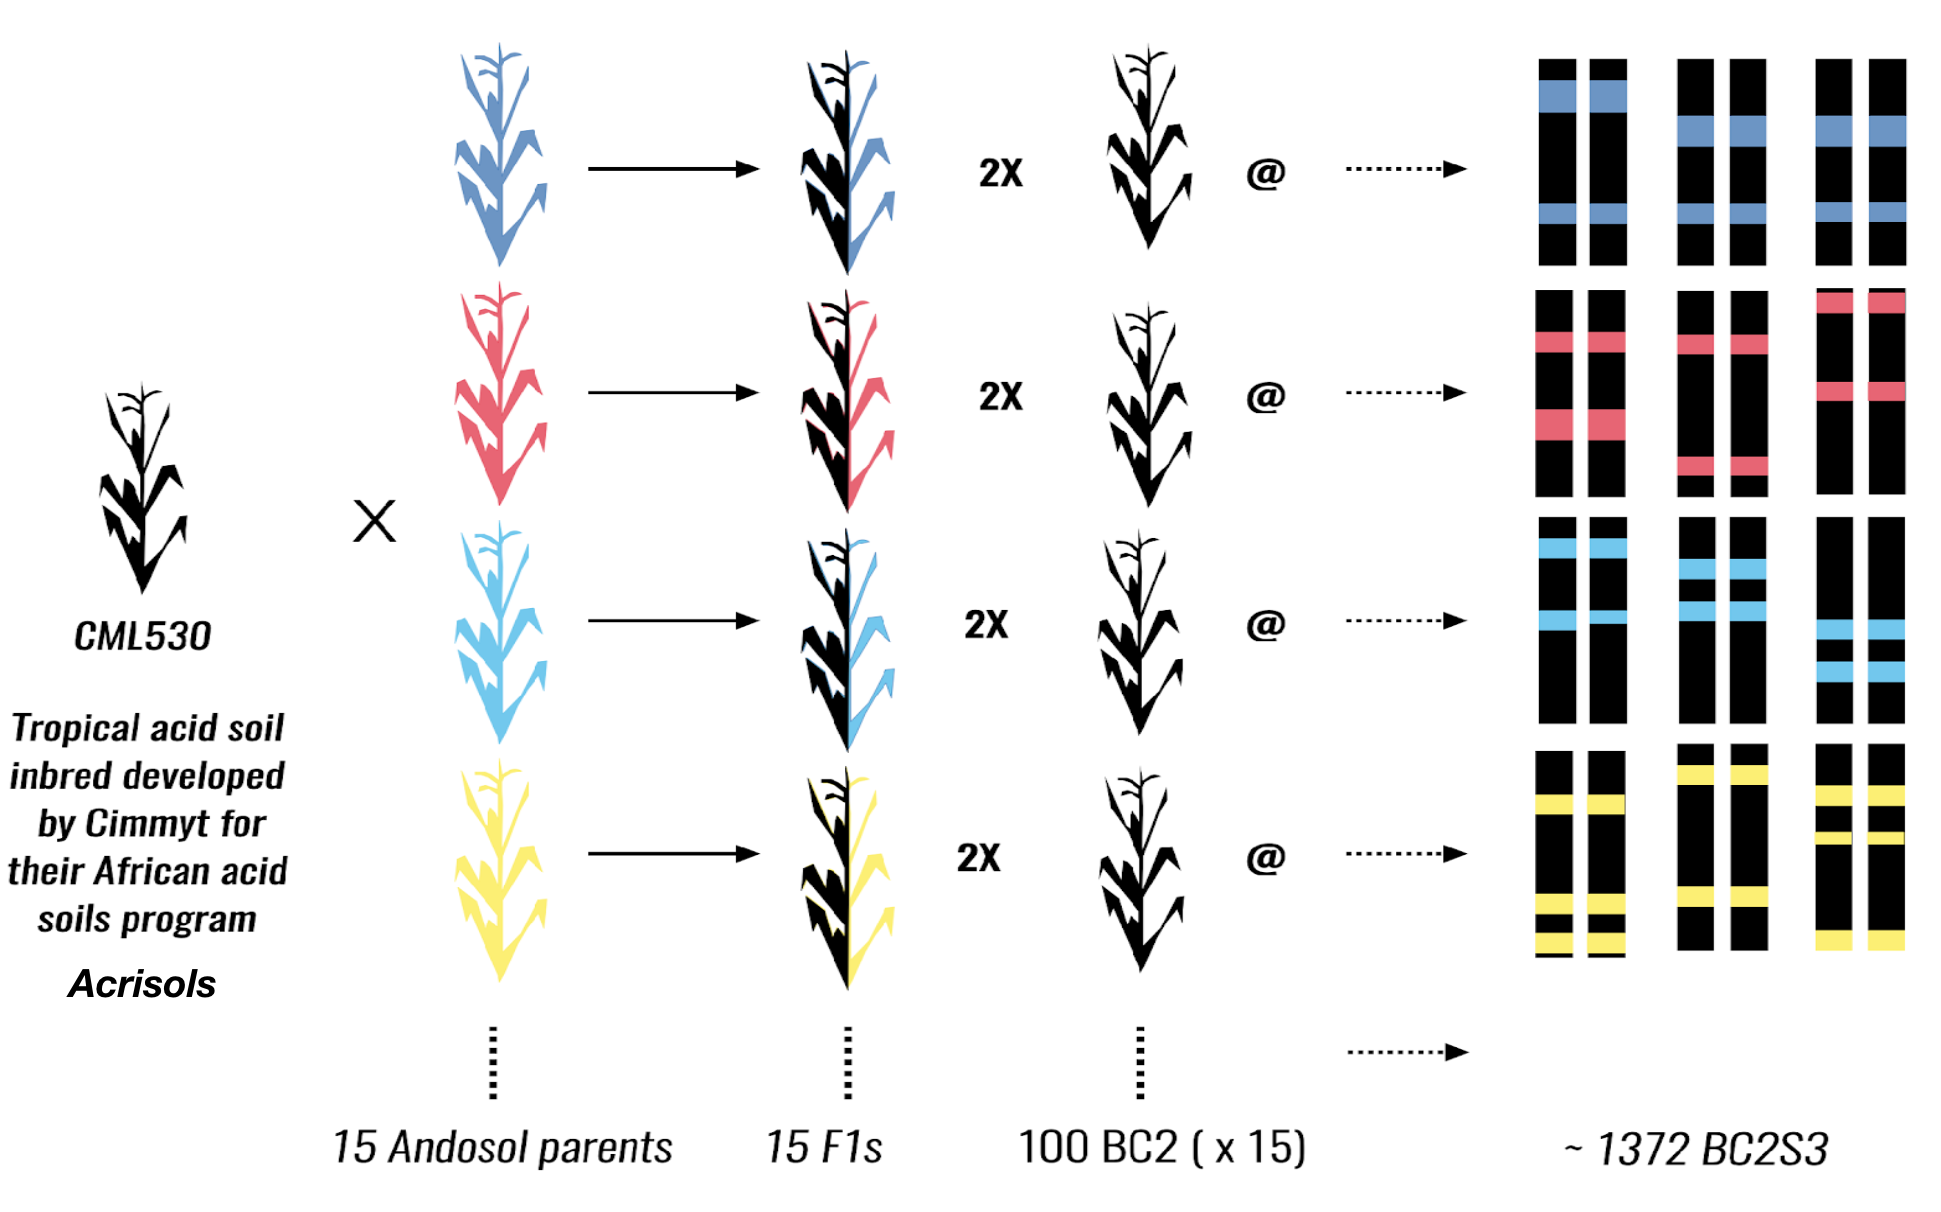
\includegraphics[width=\linewidth]{Chapter-4/figs/AIR_design.png}
\caption[ AIR Panel (Andosol Introgression Resource) Breeding scheme]
{\textit{{\textbf{AIR Panel (Andosol Introgression Resource) Breeding scheme}}}
15 landraces were selected from Mexico and Guatemala Andosols to be founders of the populations}
\label{fig::airdesign}
\end{figure}


\subsection{Inductively Coupled Plasma Mass Spectrometry (ICP-MS)}
We selected a representative kernel from each AIR line seed bulk and 
processed it for Inductively Coupled Plasma–Mass Spectrometry following the high throughput protocol described in \citep{baxter2014}.
Briefly, seeds were sorted individually in 48 well plates and weighed automatically by a custom-made robot and then transferred to 110 mm borosilicate glass test tube for digestion with 2.5 mL concentrated nitric acid overnight at 105 \textdegree C. 
After two serial dilutions of this digestion in ultra pure water (18.2M $\Omega$  Milli-Q system, Millipore) 1:4, and 0.9:4.1, a final aliquot of 1.2 mL was loaded into 96 well autosampler trays.
The samples were processed in an Agilent 7500 ICP-MS system, and the signal was adjusted to machine drift.
Collision data was collected for Al, B, Ca, Fe, K, Mg, Mn, Mo, Ni, P, S, Zn, Na, and Cu. 
The final concentrations of minerals were calculated as mg of element per kg dry seed weight.
Measurements beyond three times the interquartile range were deemed as outliers and discarded for the following analysis \citep{baxter2013}.
Additionally, quantifications for Al, B, Mo, Ni, Na, Cu, were discarded because the concentrations were too close to the detection limit of the mass spectrometer as previously reported \citep{baxter2013}.


\subsection{Genotyping}
 To genotype the BC$_2$S$_3$ families, we first sequenced the 15 F1 CML530 $\times$ Donor founder individuals and the CML530 recurrent parent using Illumina, generating an average of 30x coverage. In total, we generated ~ 85 million SNPs.
 We identified ~101,000 SNPs that were common across all F1 individuals and were heterozygous between the landrace parents and CML530. From this set of SNPs, we used plink's LD Pruning tool to select a subset of SNPs unlikely to be in linkage disequilibrium. Using a window size of 50kb and selecting 5 SNPs per window,  we obtained a final set of ~ 3,000 SNPs.
 We then designed primers for amplicon sequencing using LGC Seq-SNP technology. 
 After PCR amplification, samples are sequenced via Illumina, and then a proprietary SNP calling pipeline based on the sequence reads.
 We obtained good amplification of around 2,500 markers distributed throughout the genome, sufficient to build and saturate a genetic map using R/QTL \citep{broman2012}.
 After recovering the genotype table from LGC services, we built a VCF file selecting 1372 samples from the RIL population, and 44 samples for the Andosol parents (corresponding to 15 accessions per duplicate plus 8 other accessions not used in the crosses).
I converted the VCF file to ABH (A: recurrent, B: donor, H: heterozygote) format using a custom R script that coded any genotype different from CML530 as B (donor) genotype.
A $\chi^2$ test for goodness of fit to Mendelian segregation for a $BC_2S_3$ was used to filter distorted markers. 
However, the $\chi^2$ statistic was inflated because of a general excess of heterozygotes (observed frequency = 0.09, expected frequency = 0.03), so I decided to discard markers above the $95\%$ percentile of this empirical $\chi^2$ distribution for genetic mapping. 
Having this list of acceptable markers, I returned to the VCFs, imputed genotypes by nearest neighbor in TASSEL5 \citep{bradbury2007}, and converted once more to ABH format for QTL mapping.
The R scripts and data are reported in the public GitHub repository  \href{https://github.com/sawers-rellan-labs/airmine}{\texttt{airmine}}.


\subsection{Genetic Map, QTL Mapping, heritability estimation}
Starting with the ABH genotype table for the joint population I created a R/QTL \citep{broman2012} cross object for a BC$_2$S$_3$ population, with linkage groups and marker order according to the B73 reference AGPv4. I used the function \texttt{map} to calculate initial recombination fractions according to the expectations of this type of population. 
Subsequently, I removed markers isolated by more than 10 cM from other markers and recalculated the recombination fractions once more, for a map with a final count of 1996 markers and 1283 individuals passing quality control. 
I used the stem macro hairs and the presence of anthocyanin pigments in stems as binary (presence/absence) traits that we scored at the generation before bulking, during the summer of 2019 at the Central Crops Research Station, Clayton, NC.
For the 7 high-quality mineral traits and seed weight, I did a first round of single marker QTL search in the BC$_2$S$_3$ population, using year and donor block as covariates. 
Genome-wide LOD thresholds were established after 10000 permutations of the phenotype with respect to genotypes, and correction for multiple phenotypes.
These QTL positions were used as a starting point for a second round of QTL search by Multiple Interval Mapping (MIM) with forward and backward marker selections using the \texttt{stepwiseqtl} function. 
To shorten computing time, I picked conservative likelihood penalties (4,4,4),  relative to the R/QTLs defaults (suggested for mice), instead of making a two-marker search.  
For heritability estimation, I used a mixed model in ASReml implemented in R.
The mineral content was modeled as a function of covariates as fixed effects, year and donor block, and genotype effect at each marker as random effect.
The narrow sense heritability $h^2$ was estimated as the proportion of variance explained by the SNPs in this mixed model. 
QTL heritability was reported as the proportion of variance explained by significant QTLs found by MIM.
As an indicator of environmental variance, I calculated the proportion of variance explained by the donor/block (plots from a single donor were not randomly placed but planted in blocks) as a fixed effect in the MIM model per trait.
The R scripts and data are reported in the public GitHub repository  \href{https://github.com/sawers-rellan-labs/airmine}{\texttt{airmine}}.
\clearpage

\section{Results}

\begin{figure}[!ht]
\centering
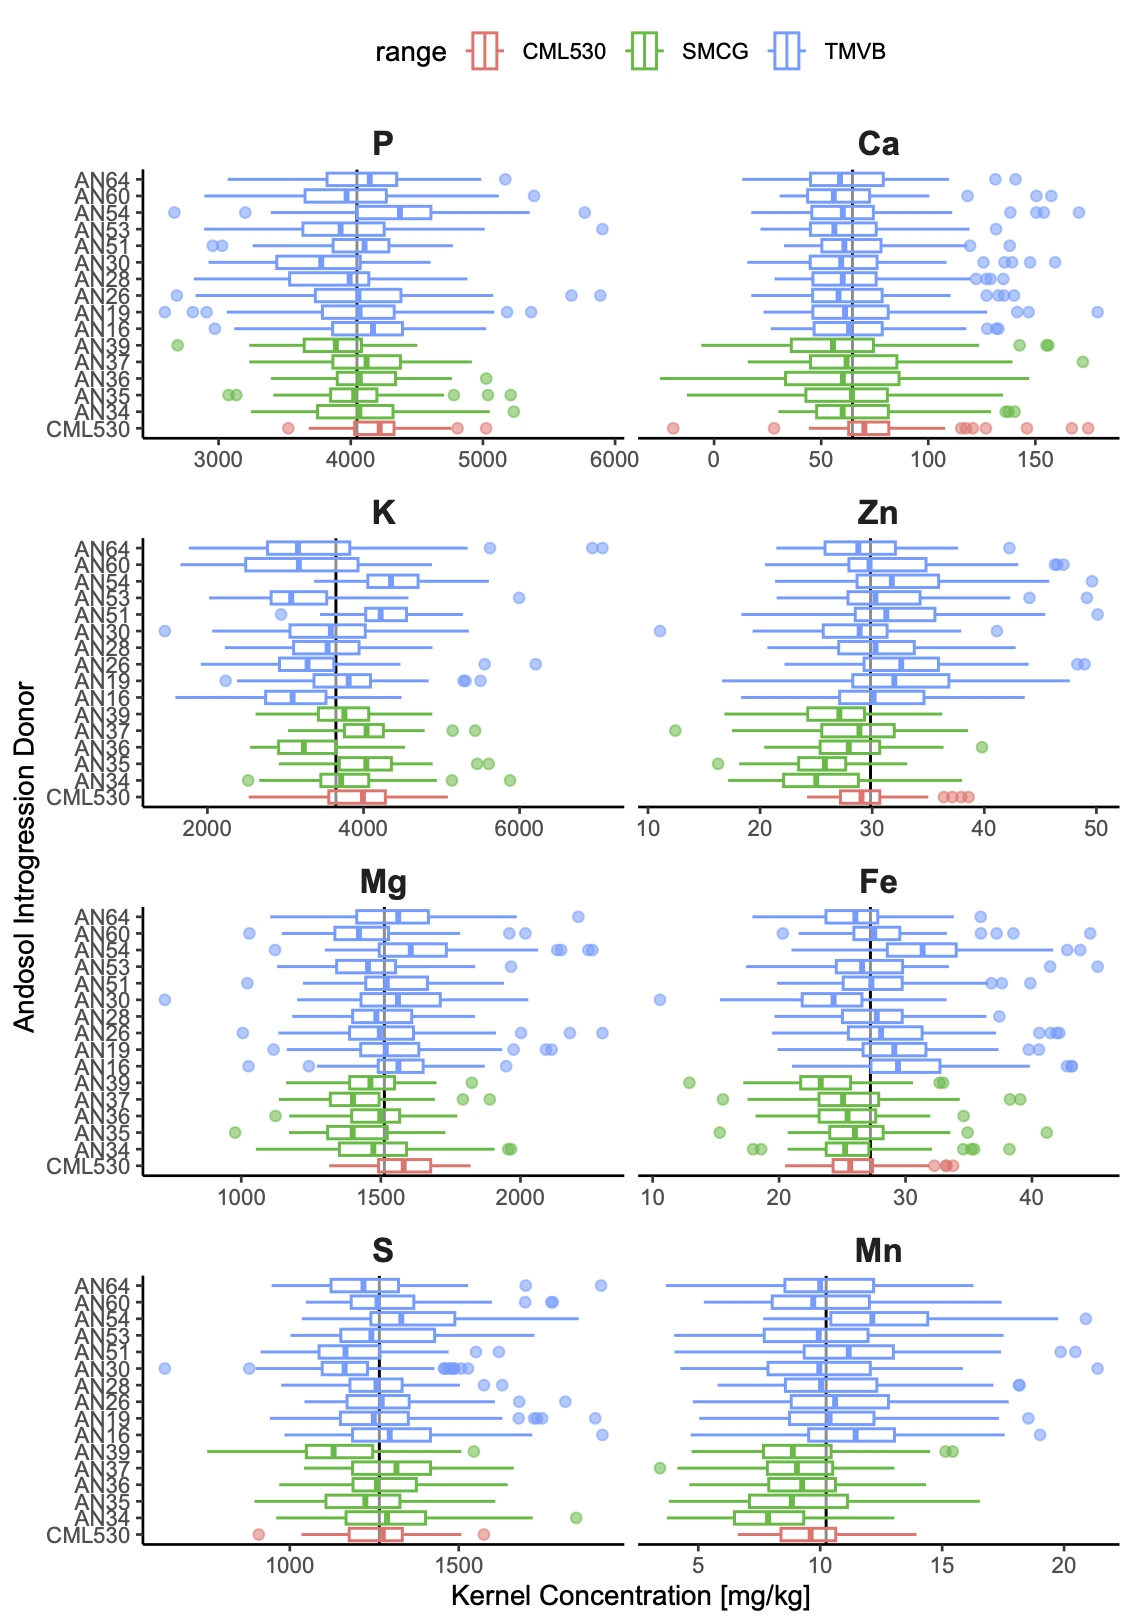
\includegraphics[width=0.8\linewidth]{Chapter-4/figs/mineral_distro.png}
\caption[Distribution of mineral kernel concentration]
{\textit{\textbf{Distribution of mineral kernel concentration.}} Minerals sorted by mean abundance from top to bottom, boxes with median, IQ range, whiskers $95\%$ quantiles. 
% Families derived from Sierra Madre de Chiapas y Guatemala (SMCG, n=375), seem to have a distinct mineral content (MANOVA, p<1e-12) than either Transmexican Volcanic Belt (TMBV, n=910, Zn, Mg, Fe, Mn), or CML530 material (n=70, Mg, Zn, Mn), however, the effect is confounded with year as the SMCG material was planted in a different season.
}
\label{fig:mineraldistro}
\end{figure}
\clearpage


\subsection{Lines descending from TMBV Andosol donors have significantly lower P, K, and Mg concentrations than CML530 checks.}

We obtained reliable measurements for 8 minerals P, K, Mg, S, Ca, Zn, Fe, and Mn. 
The kernel mineral content varied over 3 orders of magnitude with phosphorus and potassium being the most abundant (with means around 4000 ppm) while manganese showed the lowest concentrations (mean 10 ppm), (\autoref{fig:mineraldistro}). 
The first component of the mineral PCA (\autoref{fig::mineralPCA} Left), had a high contribution of P, Mg, Zn, and S, while the second component's highest contribution was from K. 
The samples showed no clustering according to mountain range in these first two, nor in higher dimensions of the PCA. 
However, material from TMVB accumulated less  P, K, and Mg than CML530 (\autoref{fig::mineralPCA} Right), even after correcting by year (linear model $\beta$ t-test  $p < 0.05$). The year of planting (2020 or 2021), did not have a significant effect on  P or K, but it did on Mg (linear model $\beta$ t-test  $p < 0.05$).

\begin{figure}[!ht]
\centering
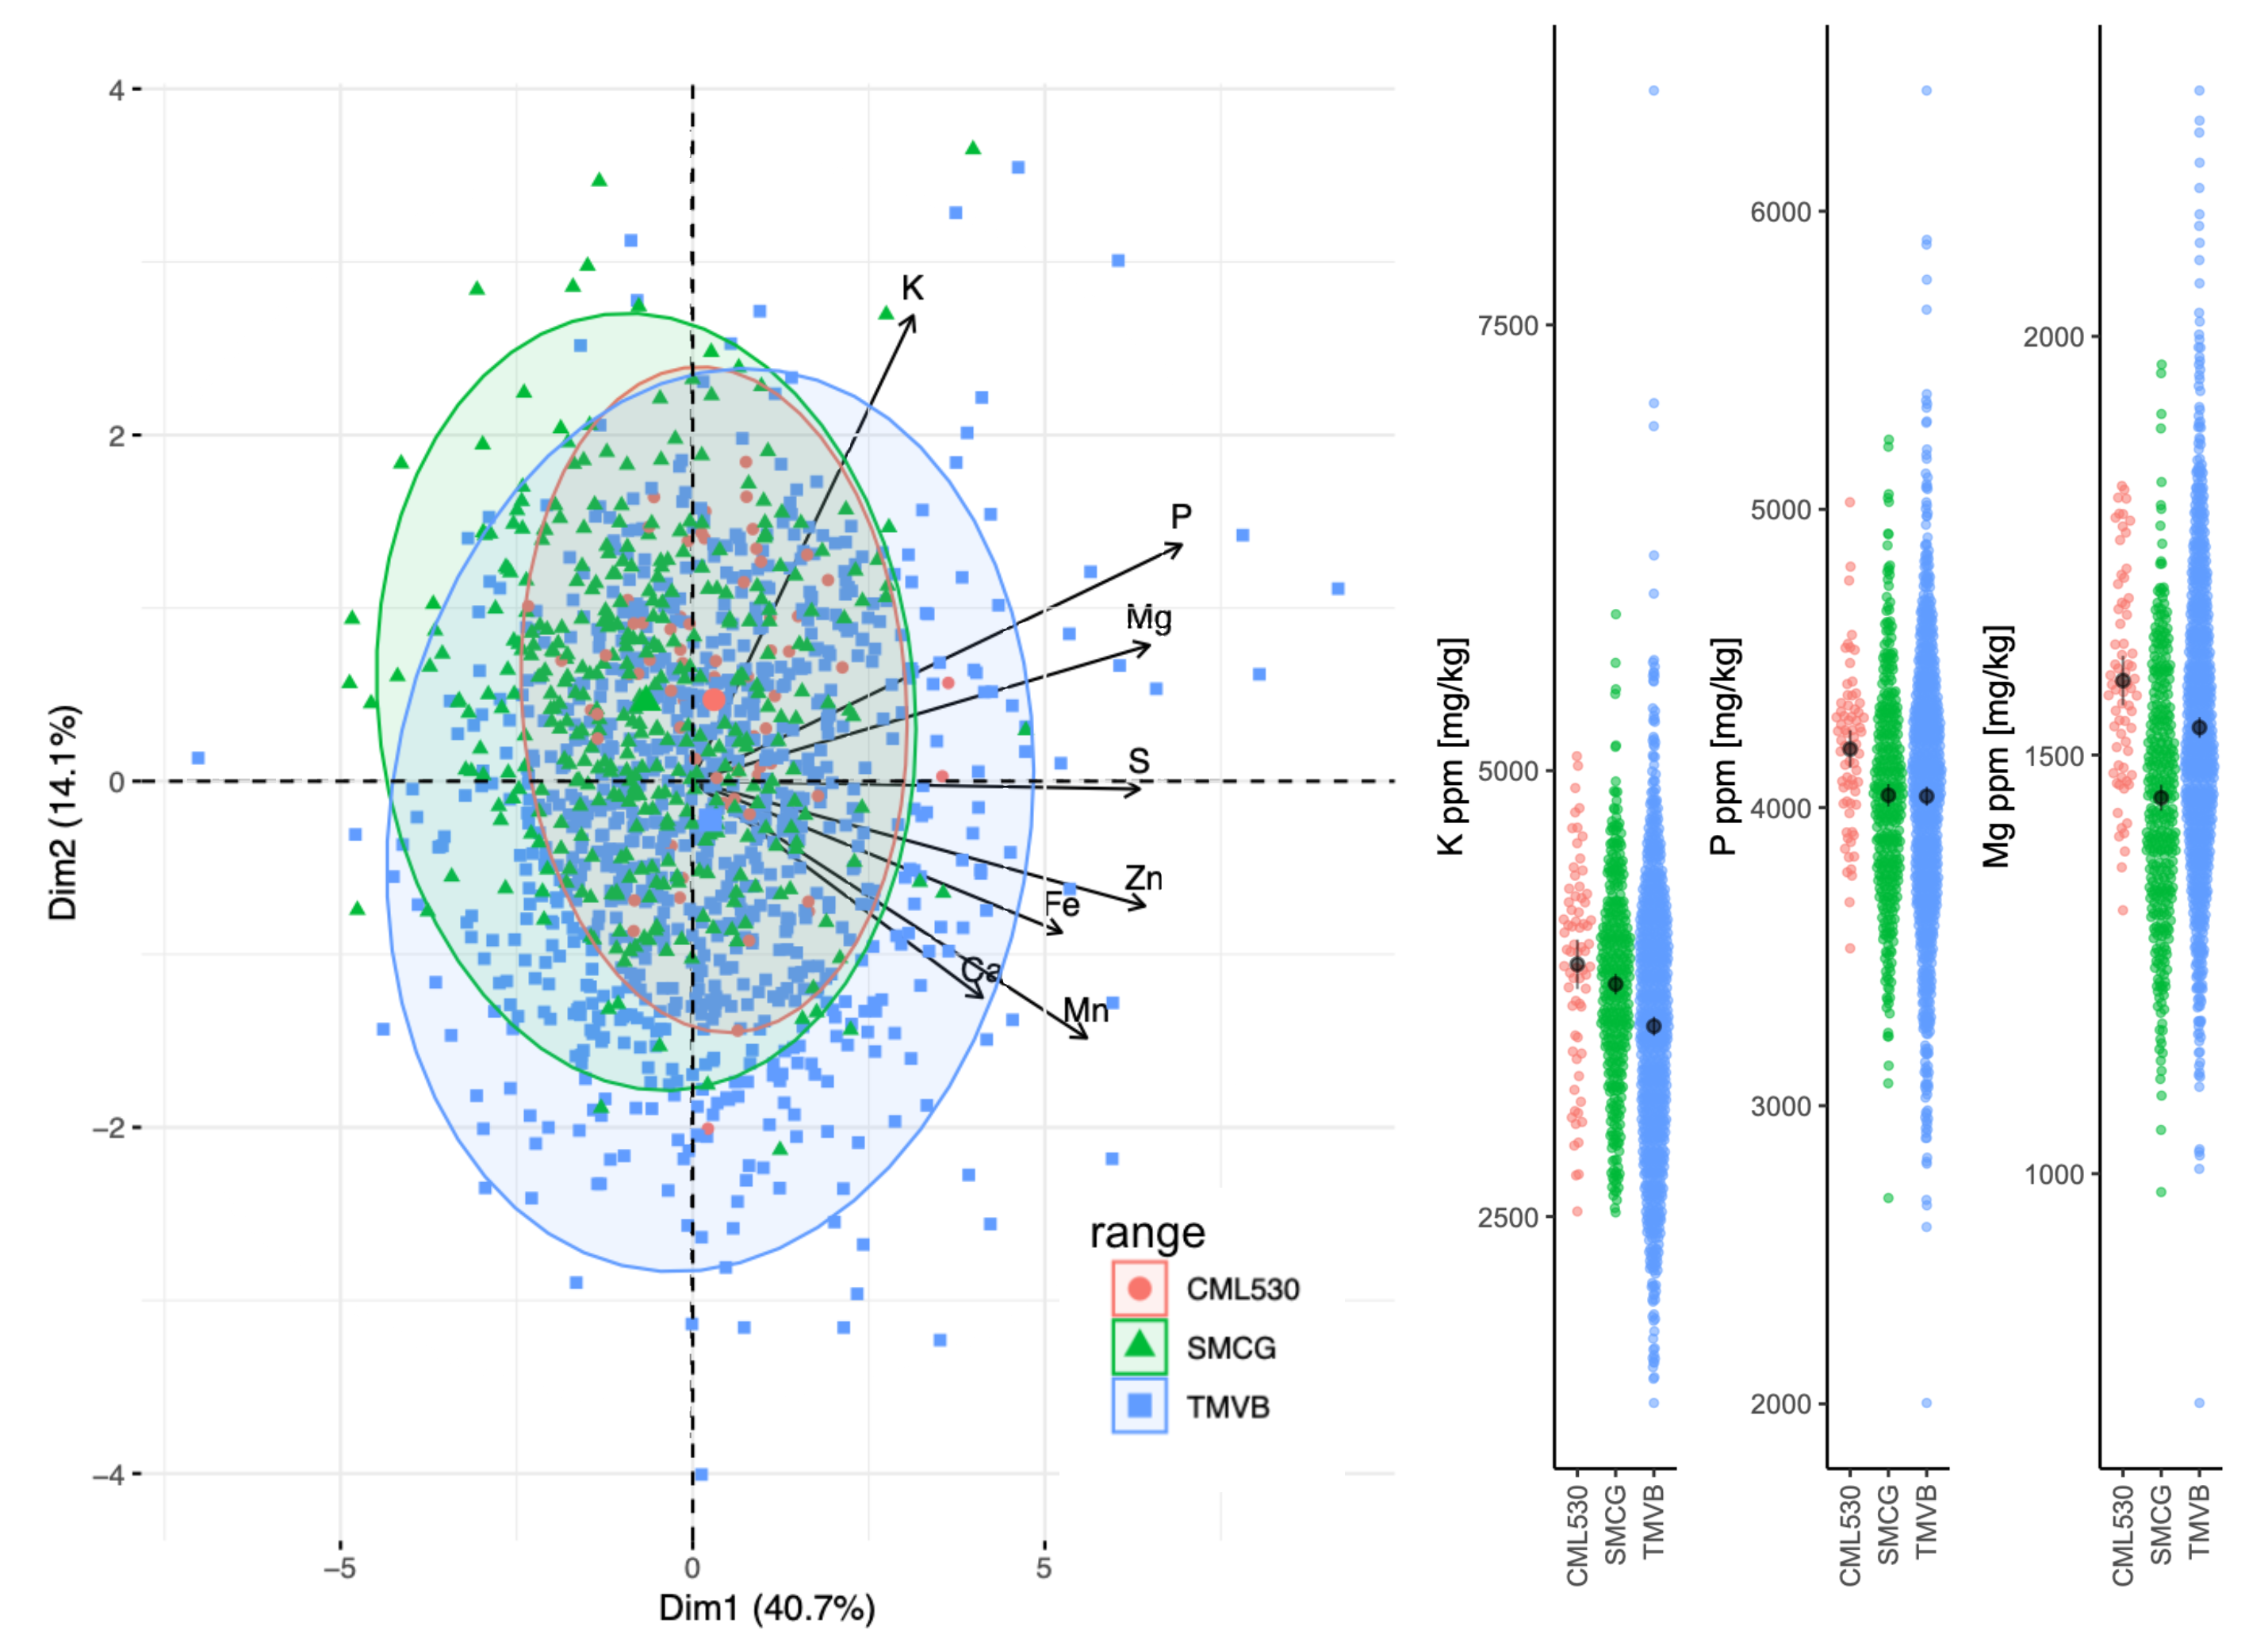
\includegraphics[width=0.9\textwidth]{Chapter-4/figs/mineral_PCA.png}
\caption[ Kernel mineral PCA shows no clustering by geographic origin but Transvolcanic Belt derived NILs differ from CML530 in K,P and Mg. ]{\textit{\textbf{Kernel mineral PCA shows no clustering by geographic origin but Transvolcanic Belt derived NILs differ from CML530 in K,P and Mg.}}. \textit{Left:} Kernel Mineral PCA. The First dimension has a high contribution from P, Mg, Zn and S; the second dimension's main contribution is from K.  
\textit{Right:} There are significant differences between the mineral composition of families derived from parents of different geographic range (SMCG and TMVB) and the recurrent parent CML530.
Mean and $95\%$ confidence intervals in black.}
\label{fig::mineralPCA}
\end{figure}
\clearpage


\begin{figure}[!ht]
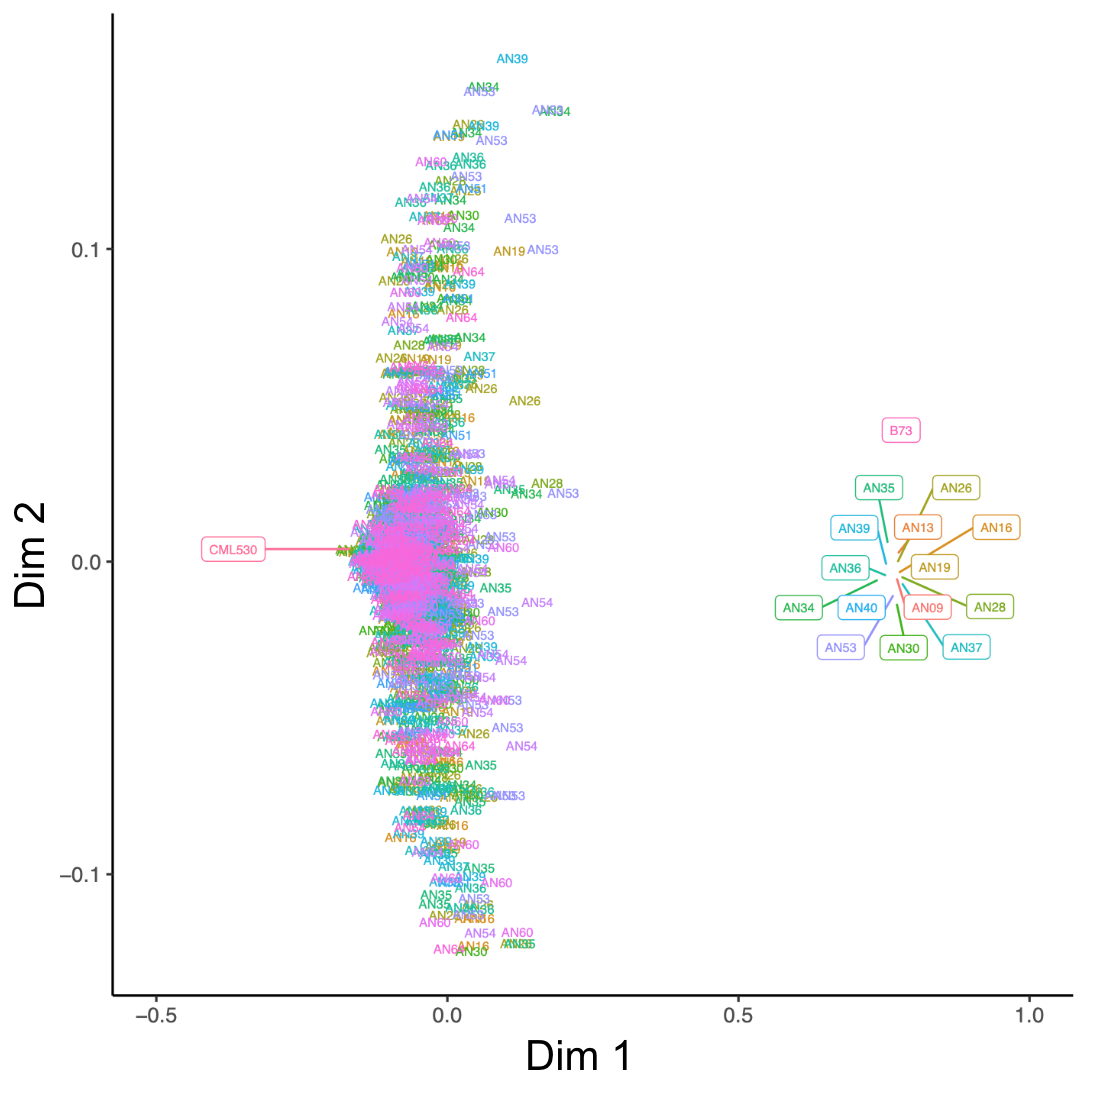
\includegraphics[width=\linewidth]{Chapter-4/figs/genetic_MDS.png}
\caption[Genetic MDS of AIR lines]{\textit{\textbf{Genetic MDS of AIR lines shows no apparent population structure.}}
Dim1 separates the recurring parent CML530,  from the Andosol Donors (labeled boxes). Dim2 shows variation inside the NILs (no boxes, each NIL labeled and colored by donor) and  separation of the Andosol parents from  B73.}
\label{fig::genetic_MDS}
\end{figure}

\clearpage

\subsection{QTL mapping on the AIR panel genetic map replicates previously detected loci associated with highland traits.}
After imputation, the genotype table had 1996 markers and 1283 individuals with 0\% missing data. 
A multidimensional scaling visualization of the genetic marker data (\autoref{fig::genetic_MDS}), shows no apparent population structure, as individuals are not clustered per Andosol donor. 
I obtained a joint genetic map with a total genetic length of  2921 cM, \autoref{fig::mineralQTL} A, and  mean distance between markers of 1.46 cM ( $\sigma = 1.63$ cM).
As a quality check, I mapped two highland maize traits \citep{ janzen2022, perez-limon2022, lauter2004} and I was able to detect significant QTLs for both, sheath purple pigmentation (LOD =29) and sheath macrohairs (LOD =22)(\autoref{fig::highland_traits}).
The QTL peaks co-localized with the previously reported loci, \textit{b1} for anthocyanins \citep{perez-limon2022,chandler1989} and \textit{mhl1} for macrohairs \citep{perez-limon2022,calfee2021-mr, moose2004} in chromosomes 2 and 9 respectively. 

\begin{figure}[!ht]
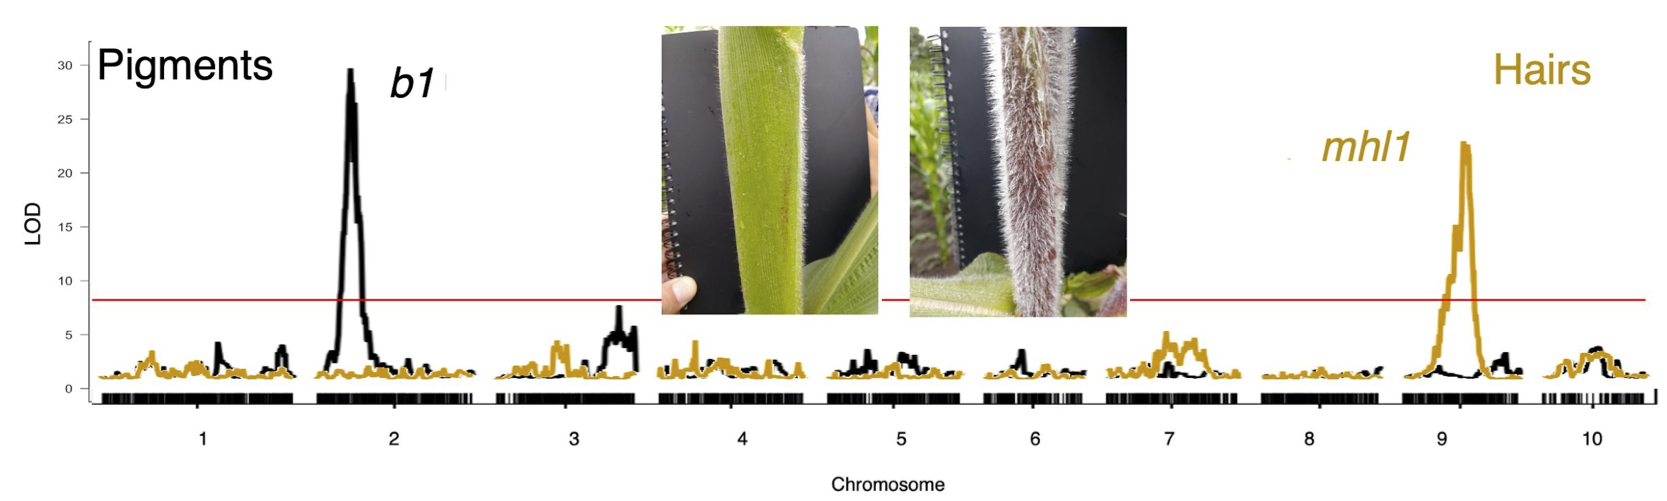
\includegraphics[width=\linewidth]{Chapter-4/figs/highland_traits.png}
\caption[QTL mapping of two highland traits]{\textit{\textbf{QTL mapping of highland traits}} Strong signals were detected for both sheath anthocyanin pigmentation and sheath macro hairs coinciding with previously reported loci \textit{b1} and  \textit{mhl1}.
}
\label{fig::highland_traits}
\end{figure}

\clearpage

\subsection{Multiple QTLs underlie kernel mineral content in the AIR population.}
In the joint QTL analysis, I found 12 genome-wide significant QTLs for all measured minerals except calcium, (\autoref{tab:mineralQTLs}). 
The QTLs explain between $1.8$ (Fe, K) to $6.6\%$ (Mg) of the observed variance in kernel mineral content. 
The most significant QTLs were found for Mg and Mn.
I detected a significant QTL for kernel phosphorus in chromosome 2 (P2@77.4, LOD = 6.3, 2.2 \% of P explained variance), which is even more significant for Mn (Mn2@77.4, LOD = 8, 2.6 \% of Mn explained variance).
RILs carrying donor alleles at Mg and P QTLs  have higher nutrient content than CML530 homozygous Lines,  (\autoref{fig::mineralQTL} right).


% Please add the following required packages to your document preamble:
% \usepackage{booktabs}
% \usepackage{graphicx}
\begin{table}[]
\caption{Kernel mineral QTLs detected in the AIR population}
\label{tab:mineralQTLs}
\resizebox{\textwidth}{!}{%
\begin{tabular}{@{}lrrrrrlr@{}}
 &
  \multicolumn{1}{l}{} &
  \multicolumn{1}{l}{} &
  \multicolumn{2}{c}{Confidence interval} &
  \multicolumn{1}{c}{} &
  \multicolumn{1}{c}{} &
  \multicolumn{1}{c}{\% varaiance} \\
\multicolumn{1}{c}{QTL} &
  \multicolumn{1}{c}{chr} &
  \multicolumn{1}{c}{cM} &
  \multicolumn{1}{c}{upper limit} &
  \multicolumn{1}{c}{lower limit} &
  \multicolumn{1}{c}{LOD} &
  \multicolumn{1}{c}{marker} &
  \multicolumn{1}{c}{explained} \\ \midrule
Mn1@186.7  & 1  & 186.7 & 185.0 & 188.5 & 23.0 & S1\_162960263  & 5.5 \\
Mg10@120.5 & 10 & 120.5 & 115.9 & 122.5 & 17.7 & S10\_115012063 & 6.6 \\
Mn3@209.2  & 3  & 209.2 & 205.5 & 210.6 & 12.2 & S3\_187045311  & 3.7 \\
Mg9@225.8  & 9  & 225.8 & 221.6 & 234.1 & 12.1 & S9\_152689448  & 4.3 \\
Mn2@77.4   & 2  & 77.4  & 74.3  & 83.7  & 8.0  & S2\_26044693   & 2.6 \\
S3@212.8   & 3  & 212.8 & 209.2 & 215.3 & 7.7  & S3\_191225238  & 2.8 \\
Zn1@372.5  & 1  & 367.1 & 364.3 & 372.5 & 7.3  & S1\_306777881  & 2.5 \\
Fe3@197.7  & 3  & 197.7 & 192.8 & 203.3 & 6.8  & S3\_180833171  & 1.9 \\
Fe7@68.1   & 7  & 68.1  & 63.9  & 75.9  & 6.7  & S7\_18152924   & 1.8 \\
Mn2@33.0   & 2  & 33.0  & 22.2  & 46.2  & 6.4  & S2\_6439011    & 2.3 \\
P2@77.4    & 2  & 77.4  & 74.3  & 79.1  & 6.3  & S2\_26044693   & 2.2 \\
K4@45.5    & 4  & 45.5  & 36.0  & 54.8  & 5.3  & S4\_10806637   & 1.8
\end{tabular}%
}
\end{table}


%QTLs that were found in the joint analysis but not in the per family analysis

% Family specific QTLs.

% QTLs  showing matching  effect sign through families

% QTL showing incongrouent signs between families

\begin{figure}[!ht]
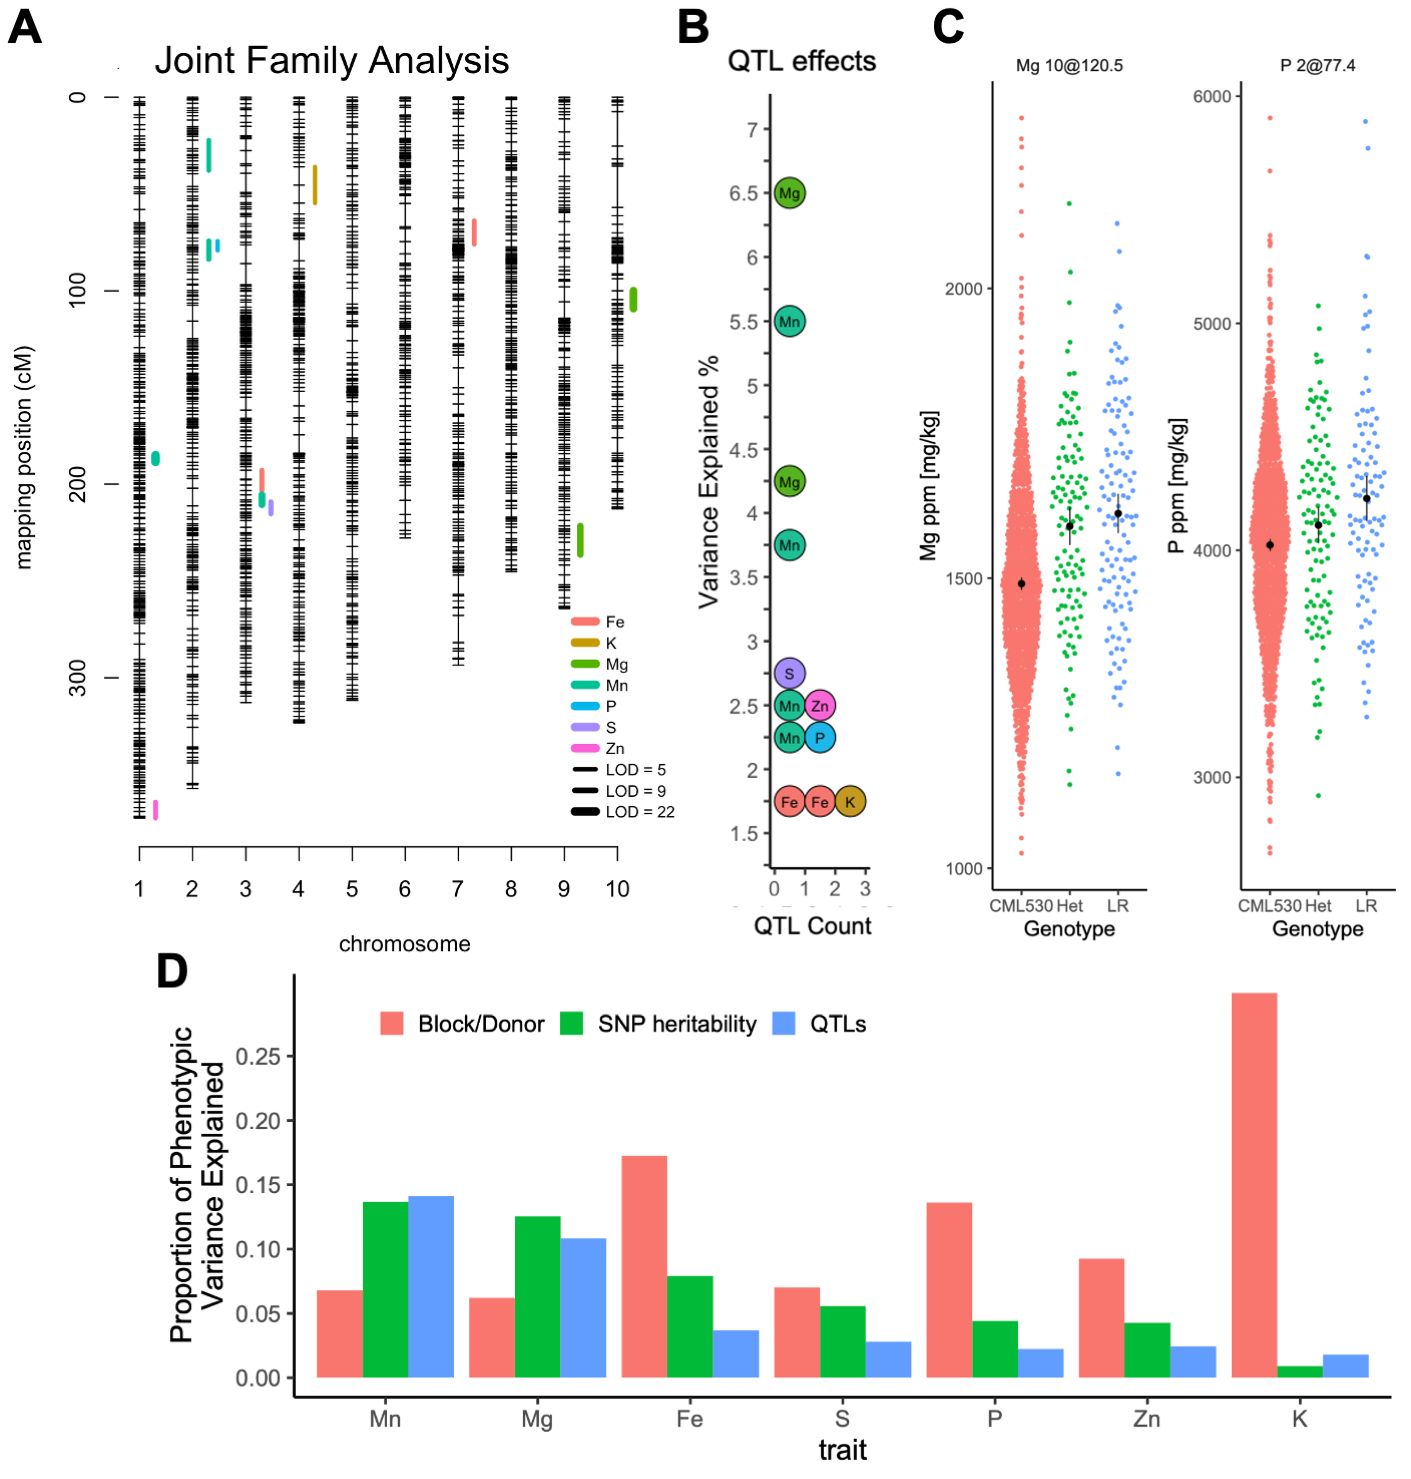
\includegraphics[width=\linewidth]{Chapter-4/figs/mineral_qtls.png}
\caption[Kernel Mineral QTLs for the AIR panel]{\textit{\textbf{Kernel Mineral QTLs for the AIR panel}}
\textbf{(A)} Significant QTLs in joint mapping analysis.
\textbf{(B)} QTL effects as percentage of observed variance in the mineral content. 
\textbf{(C)} QTL effect sizes, as ppm, for Mg, largest observed effect, and P. 
CML530, recurrent parent homozygous.
Het, heterozygous.
LR, Andosol donor homozygous.
\textbf{(D)}  Phenotypic Variance Contributions. 
Comparison of variance contributions in separate models.
QTL contribution is calculated from the MIM models.
Narrow sense SNP heritability ($h^2$) estimated from variance components of a genomic relationship animal model implemented in ASReml.}


\label{fig::mineralQTL}
\end{figure}
\clearpage

\begin{figure}[b]
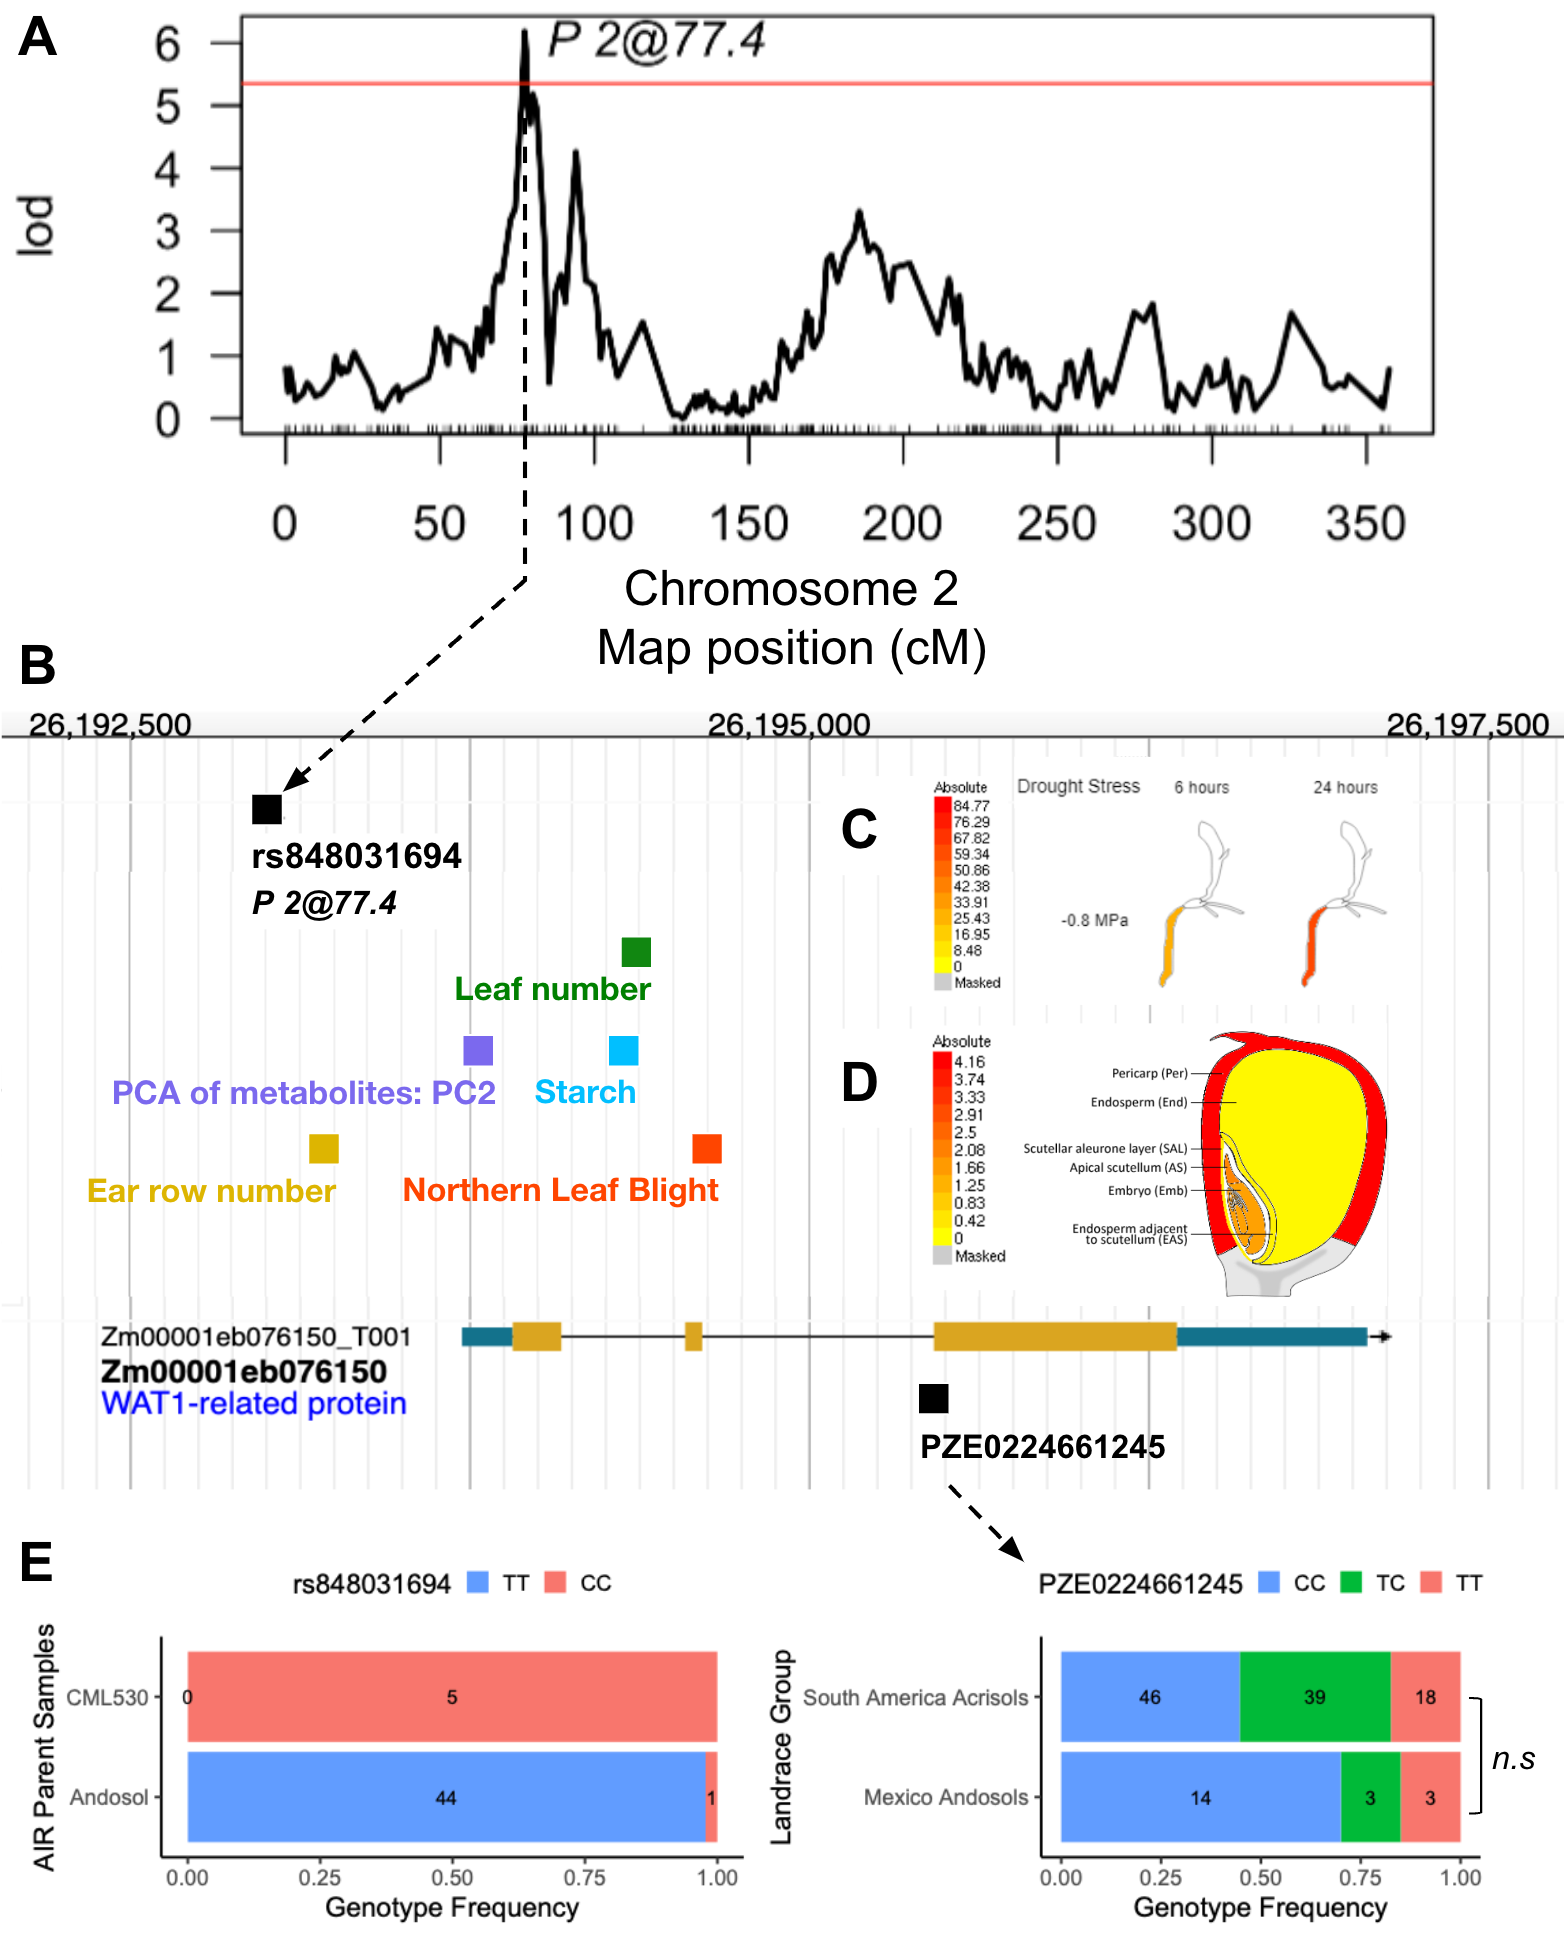
\includegraphics[width=\linewidth]{Chapter-4/figs/WAT1.png}
\caption[]{}
\label{fig::WAT1}
\end{figure}

\clearpage

\addtocounter{figure}{-1}
\begin{figure} [t!]
  \caption[Kernel Phosphorus QTL genomic context]{\textit{\textbf{Kernel P QTL genomic context.}} \textbf{(A)} MIM LOD profile for phosphorus at Chr 2, P2@77.4 is the QTL peak marker (rs848031694).
  \textbf{(B)} rs848031694 is ~1500 bp upstream of WAT1 an auxin transporter showing GWAS associations with several phenotypes under phosphorus sufficiency (colored tracks). It is highly expressed in the pericarp \textbf{(C)} and embryonic root under \textbf{(D)} drought stress .
  %This region also shows signals of selection during maize domestication/improvement, which most likely means that some specific alleles from teosinte were recruited to cultivated maize at this site. 
  \textbf{(E)} Although there is an intronic SNP in \textit{WAT1} that has an allelic frequency higher in a sample of Mexican Andosol landraces compared with  South American Acrisols (where the recurrent parent was bred) it shows no significant evidence of selection according to soil type.}
\end{figure}

\section{Discussion}
In this study, we took advantage of the seed bulks prepared during the development of the Andosol Introgression Resource panel to measure kernel minerals under optimal agronomic conditions in our winter nursery in Puerto Vallarta, Mexico.
The donor founders and the recurrent parent had been selectively bred in different soils, a humic acrisol for the recurrent parent CML530, and various types of andosols for the donors.
Although physicochemically distinct, both types of soils have high phosphorus retention \citep{batjes2011,bayuelo-jimenez2011}, and, most relevant for plant phosphorus physiology, both tend to have low phosphorus availability in the absence of fertilizer.
For example, four pine forest andosols from the Purépecha Plateau in Mexico are reported to have 0.9-8 ppm Bray-1 P [mg P/kg dry soil] \citep{galvan-tejada2014} and the natural soil P content in the humic acrisol where CML530 was bred is 5 ppm Bray-1 P \citep{granados1995}. 
For comparison, the minimal amount recommended for growing commercial hybrid corn in the USA is 15 ppm of Bray-1 P \citep{lyons2023}.
Both andosols and acrisols are acid soils, but they differ critically in mineral composition, as the latter has higher clay content due to increased weathering, and a more advanced stage of paedomorphosis, among other differences \citep{hexianjin2022,batjes2011, wrb2022}.

As an experimental segregating population, we assume that a detectable part of the observed variability in kernel mineral accumulation of the AIR panel lines must be genetic.
So we intended to look for the underlying loci for seed mineral content by linkage mapping of the different mineral traits in a common garden.
However, this study is more of an observational nature than a randomized experiment. 
Plants derived from a single donor were grown close together forming blocks, and subpopulations from donors of different mountain ranges (TMBV vs SMCG) were planted in different years (2020, 2021). 
This results in two confounding variables that I corrected for when modeling the response of the kernel mineral content as a function of the plant genotypes: donor block and year. 
After correcting for the covariates I was still able to detect 12 QTLs for 7 kernel minerals in the AIR panel (\autoref{tab:mineralQTLs} and \autoref{fig::mineralQTL}).
As we sampled a single kernel per line with no replicates we can not estimate broad sense heritabilities from variance components, because we have no estimate of the environmental variation of kernel seed content for a single genotype.
However we 1) estimated narrow sense heritabilities based on a mixed model that included the SNP-based genomic relationship matrix of the population and 2) estimated the contribution of field spatial heterogeneity as the donor block factor.
We see that the contribution of spatial heterogeneity/donor parent factor is greater than $h_{SNP}^2$ for 5 out of the 7 minerals with QTLs, (\autoref{fig::mineralQTL} D). 
More than 25\% of the variation in kernel K content might be explained  by the donor block factor, making it the mineral most influenced by potential field heterogeneity, e.g. uneven K fertilization, and/or andosol donor founder, while Mn and Mg were less influenced by this effect.
MIM QTL estimated contribution was higher than SNP heritability for Mn and K. 
In the case of magnesium, the SNP heritability excess is slight, but the similarity of the two estimators suggests that the genetic contributions for Mn content were essentially captured by the 3 detected loci, Mn1@186.7, Mn3@209.2, and Mn2@77.4. 
In general, no $h_{SNP}^2$, surpassed 15\% for any mineral, while previously reported narrow sense heritabilities in a B73 x IL14H population varied between 28\% (Na) and 81\% (P) \citep{baxter2014} in single environments.  
This indicates sources of unaccounted variance during the experiment and mineral measurements.

Nevertheless, I found a phosphorus QTL, of minor effect, in chromosome 2, P2@77.4, explaining 2.2\% of the observed variance in seed phosphorus content. 
This 2.2\% of total P variance corresponds roughly to half of the SNP-based narrow sense heritability ($h_{SNP}^2=4.2\%$) for that trait, (\autoref{fig::mineralQTL}).

The nearest marker to P2@77.4 is the SNP rs84803164 at 26044693 bp, just 1.5 kb in the promoter region of \textit{Zm00001eb076150}, a homolog to the \textit{Arabidopsis} auxin transporter \textit{WAT1} (\autoref{fig::WAT1} A). \textit{WAT1} determines secondary cell wall thickness of wood fibers in \textit{Arabidopsis} \citep{ranocha2013}. 
Several maize variants at this locus are associated with multiple phenotypes in GWAS studies, (\autoref{fig::WAT1} B).
These include leaf number under phosphorus deficiency  \citep{xu2018a}; and under phosphorus sufficiency, metabolites, starch, ear row number and resistance to northern leaf blight \citep{wallace2014a}. 
Additionally, a homolog of \textit{WAT1} in wheat has been found to be associated with shoot dry weight under low phosphorus \citep{dharmateja2022}. 
\textit{Zm00001eb076150} is expressed in the seed pericarp (\autoref{fig::WAT1} C), and is overexpressed in the primary seminal root under drought stress  (\autoref{fig::WAT1} D). 
The overlap of P2@77.4 and Mn2@77.4, might point to a single locus of pleiotropic effect. Mn and P have been shown to co-accumulate in leaves of plants that rely on carboxylates for nutrient mobilization \citep{lambers2015b}, which makes it another plausible mechanism for the action of the locus.

If the donor allele at rs84803164 is related to adaptation to andosols, one would expect an increased frequency of the donor allele in traditional varieties from andosols relative to that found in acrisol adpated plants. 
I could not find genotype data for rs84803164, but I found a Zm00001eb076150 
intronic SNP, PZE0224661245, in the genotypes of \citep{romero_navarro2017-cn}.
Given the absence of acrisol varieties in Mexico in this data set,  I calculated allelic frequencies at  PZE0224661245 for two groups of traditional varieties, one from Mexican andosols and another from South American acrisols.
The C allele at this site has a higher frequency in the Mexican andosols group corresponding to the allelic pattern at rs84803164 in the AIR population founders (\autoref{fig::WAT1} E).
However, the difference between the traditional varieties of the two soil classes is not significant showing no evidence of selection at this locus.

\clearpage

\printbibliography[heading=subbibintoc, title=References]
